\documentclass[tikz,border=8pt]{standalone}
% Shared TikZ style for synorg platform diagrams. Each diagram \input's this
% inside a standalone document. Palette tracks the Material "teal" site theme so
% figures read as one system in light mode (SVGs are theme-neutral otherwise).
\usetikzlibrary{arrows.meta,positioning,shapes.geometric,fit,backgrounds,calc,decorations.pathreplacing}

\definecolor{synteal}{HTML}{00897B}   % primary
\definecolor{synfill}{HTML}{E0F2F1}   % light fill
\definecolor{synamber}{HTML}{B26A00}  % warning / lend
\definecolor{synred}{HTML}{B00020}    % deny / danger
\definecolor{syngrey}{HTML}{5F6368}   % muted

\tikzset{
  >=Stealth,
  font=\sffamily\small,
  box/.style={draw=synteal,line width=0.6pt,rounded corners=2pt,fill=synfill,
              inner sep=5pt,align=center},
  plane/.style={draw=synteal,line width=0.8pt,rounded corners=3pt,fill=synfill,
                inner sep=8pt,align=center},
  state/.style={draw=synteal,line width=0.7pt,circle,fill=synfill,inner sep=3pt,
                minimum size=11mm,align=center,font=\sffamily\footnotesize},
  decision/.style={draw=synteal,line width=0.7pt,diamond,aspect=2,fill=synfill,
                   inner sep=1pt,align=center,font=\sffamily\footnotesize},
  deny/.style={draw=synred,fill=synred!8,text=synred},
  warn/.style={draw=synamber,fill=synamber!10},
  flow/.style={->,line width=0.6pt,draw=syngrey},
  flowlbl/.style={font=\sffamily\footnotesize,text=syngrey,inner sep=2pt},
  note/.style={font=\sffamily\footnotesize\itshape,text=syngrey},
}

\begin{document}
% Strangler migration behind one shared ALB (service-migration.md): traffic
% shifts from the ECS target group to the EKS golden-chart target group by
% weight, and rollback is a weight flip back. ECS stays warm until conversion
% is proven, so the rollback path is always available.
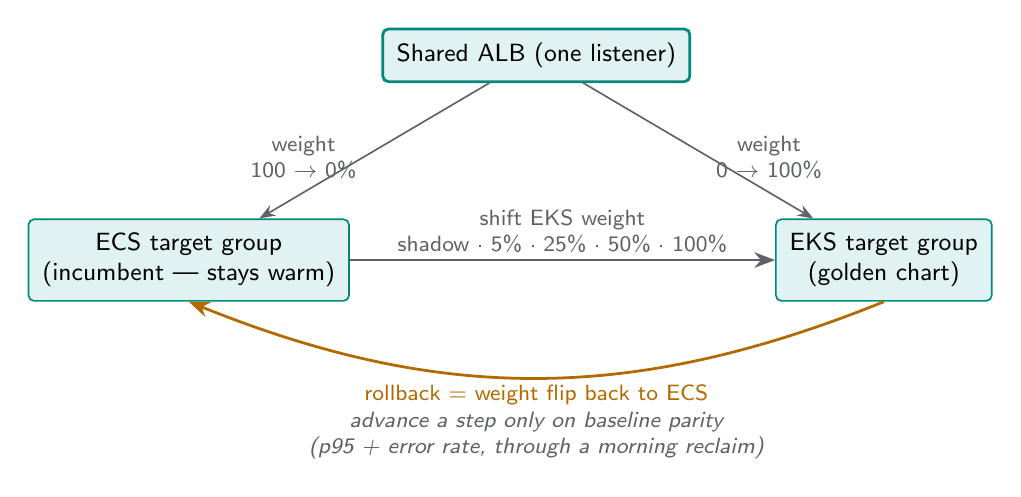
\begin{tikzpicture}
  \node[box,align=center] (ecs) {ECS target group\\(incumbent --- stays warm)};
  \node[box,align=center,right=54mm of ecs] (eks) {EKS target group\\(golden chart)};
  \node[box,line width=1pt] (alb) at ($(ecs)!0.5!(eks)+(0,26mm)$)
    {Shared ALB (one listener)};

  \draw[flow] (alb) -- node[flowlbl,left,align=center,pos=0.55]{weight\\100 $\to$ 0\%} (ecs);
  \draw[flow] (alb) -- node[flowlbl,right,align=center,pos=0.55]{weight\\0 $\to$ 100\%} (eks);

  % forward weight shift (label above the straight arrow)
  \draw[flow,line width=1pt] (ecs.east) -- node[flowlbl,above,align=center]
    {shift EKS weight\\shadow · 5\% · 25\% · 50\% · 100\%} (eks.west);
  % rollback = weight flip back (bows below, label below)
  \draw[flow,draw=synamber,line width=1pt] (eks.south) to[bend left=22]
    node[flowlbl,below,text=synamber]{rollback = weight flip back to ECS} (ecs.south);

  \node[note,align=center] at ($(ecs.south)!0.5!(eks.south)+(0,-17mm)$)
    {advance a step only on baseline parity\\(p95 + error rate, through a morning reclaim)};
\end{tikzpicture}
\end{document}
